\Chapter{Software Requirements Specification}

\section{External Interfaces Requirement}

\subsection{Hardware Interfaces}

The application is hosted in the Heroku application cloud service. The Web server communicates over HTTPS to ensure that data transferred between client and server is untampered and private. The system is a Web based application; users are required to use a high-speed Internet connection and use an up-to-date Web browser.

\subsection{Software Interfaces}

Javascript will be implemented throughout the website in order to display the correct feature the user requested. And HTML5 may be implemented throughout the website in order to display the correct feature the user requested.

\subsection{Communication Interfaces}

This application is designed to be viewed on any Internet Web browser provided that Javascript and image features are enabled and the browser is HTML5 compatible. Performance may vary slightly between browsers; however, the functionality of the site should not be impaired.

\section{Functional Requirement}

The functions specified in this section directly correspond to work that will be conducted in this project as shown in the use case diagram in Figure ~\ref{fig:use_case}. 

\vspace{3em}
\begin{figure}[H]
\begin{center}
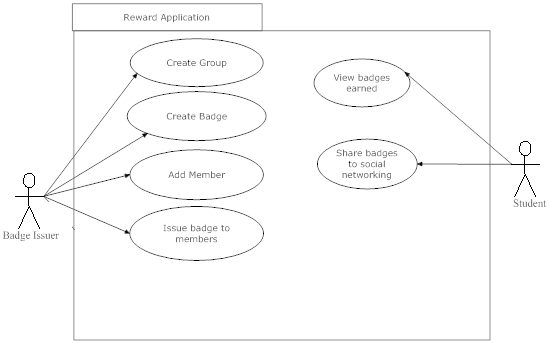
\includegraphics[height=3.8in,width=6.5in]{images/UseCase.png}
\caption{Use Case Diagram}
\label{fig:use_case}
\end{center}
\end{figure}

\subsection{Create group}

This functionality allows organizers or badge issuers to create groups, which will have a set badge collection.

\subsection{Create Badge} 

This functionality allows badge issuers to create badge to be added to badge collection. A badge would have at least badge name and description.

\subsection{Add Member}

This functionality would allow organizers or badge issuers to add members into the groups as badge recipients. Member would have at least email address and name.

\subsection{Issue Badges to Members}

This functionality would allow badge issuers to issue badges to members. 

\subsection{View Badge Earned}

This functionality would allow badge recipients to view all the badges that they have earned.

\subsection{Share Badge to Social Networking} 

This functionality would allow badge recipients to share the badge to their social networking site such as Facebook

\section{Performance Requirement}

This application is going to be hosted in the Heroku cloud server, so the performance of this application would be high.
 
\section{Design Constraint}

This application requires internet-enabled devices and internet connection to perform. And every user must have Facebook account to be able to use this. 

\section{Software System Attributes}

The author will maintain the established coding standards throughout the duration of the project (including proper commenting and documentation).
